\documentclass[a4paper, 12pt]{article}

\usepackage{a4,amssymb,color,graphicx}

\usepackage[ngerman]{babel}
\usepackage[T1]{fontenc}
\usepackage{ae,aecompl}
\usepackage[utf8]{inputenc}
%zum kuerzen
\usepackage{cancel}
%\usepackage{wrapfig}
\usepackage{fancyvrb}
\usepackage{amsmath}
\usepackage{amstext}
\usepackage{epstopdf}

%huebsche kopfzeilen
\usepackage{fancyhdr}
\pagestyle{fancy}
%\fancyhead[C]{}
%\fancyfoot[C]{}
%\fancyfoot[RE]{\thepage}
%\fancyfoot[LO]{\thepage}
\renewcommand{\headrulewidth}{0.4pt}
\renewcommand{\footrulewidth}{0.4pt}
\textheight=580pt

\bibliographystyle{plain}
%caption centern
\usepackage{ccaption}
\captionstyle{\centerlastline}
%Unterobjekte
\usepackage{subcaption}

\usepackage{hyperref}

\newcommand{\mensch}[1]{\textsc{#1}}	% Wichtige Physiker
\newcommand{\D}{\mbox{d}}				% Fuer gerade d in dx/dy
\newcommand{\VE}{\boldsymbol} %Für fette Vektoren

%%Vor dem drucken unbedignt auskommentieren -> reine bildschirmschrift - liest sich besser ;)
%\renewcommand{\familydefault}{phv}
\begin{document}

 \begin{titlepage}
 \begin{figure*}[t]
 
\includegraphics[height=2cm]{georg} \hfill
 \end{figure*}

\normalsize
\vspace{1cm}

\begin{center}
\Large Master Forschungspraktikum \\ \vspace{1cm}
\hrule \vspace{3mm}
\large {BK.MDS} \\
\Huge{\bf Molekulardynamik-Simulationen}
\vspace{5mm}
\hrule
\end{center}

\normalsize

\begin{table}[!h]
\begin{center}

  \begin{tabular}{ll}
  Praktikanten: &Philip Marszal\\
   &\\
  Betreuer: & \\
  &\\
  Gruppe: &\\
  &\\
  Durchgeführt: &\\

\vspace{1cm}& \\
  E-Mail: & \ttfamily philip.marszal@stud.uni-goettingen.de\\
\end{tabular}
\end{center}
\end{table}
\vspace{2cm}


\end{titlepage}

\thispagestyle{empty}
\newpage
\thispagestyle{empty}
\mbox{}
\newpage
\thispagestyle{empty}
\tableofcontents
\newpage

\pagestyle{fancy}
\setcounter{page}{1}

\section{Einleitung}
%Wofür wird MDS gebraucht?
%Bedeutung von Proteinbewegungen.
%Ziel des Versuches

\section{Theorie}
%Einleitung mit Motivation des Versuchs, Vergleich zu anderen hochauflösenden
%Mikroskopietechniken mit Literaturrecherche (ca. 1 Seite).
\subsection{Lichtmikroskopie}
STED-Mikroskopie ist eine Form der Lichtmikroskopie, die eine besonders gute Auflösung erreicht im Vergleich zu klassischen Mikroskopen.
Das klassische Lichtmikroskop basiert auf einem simplen Aufbau aus Linsen, wie er für einen einfachen Fall in Abb. \ref{fig:lightmic} zu sehen ist.
\begin{figure}
	\centering
	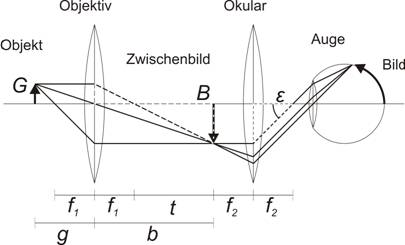
\includegraphics[width=0.6\textwidth]{plots/micro.jpg}\caption{Schematische Darstellung eines Zwei-Linsen Mikroskops aus. (Quelle: https://wiki.physik.fu-berlin.de)}\label{fig:lightmic}
\end{figure}
Im simpelsten Fall besteht wirft die erste Linse, das Objektiv, ein Bild in die Fokusebene der zweiten Linse, dem Okular \cite{Dem2}.
Der kleinst mögliche Abstand zweier Punkte unter dem noch zwei getrennte Punkte erkannt werden können ist die Auflösung des Mikroskops.
Sie ist bei der Lichtmikroskopie grundlegend durch Beugung beschränkt.
Beugung bewirkt, dass das Bild eines Punktes kein weiterer Punkt ist sondern eine mithilfe der Besselfunktion beschriebene Verteilung konzentrischer Ringe \cite{Born}, die sogenannte Punktspreizfunktion (PSF, \emph{point spread function}).
Insbesondere hat das Zentrum der Ringe, das erste Maximum, eine endliche Ausdehnung.
Dieses erste Maximum wird im Allgemeinen als Arrayscheibe bezeichnet.
\\
Das mit einem Mikroskop aufgenommene Bild einer Probe entspricht in seiner Form der Faltung der realen Form der Probe mit der PSF des Mikroskops.
Auf eine scharfe Kante wirkt diese Faltung als Glättung, sodass im Bild nur ein gradueller Übergang zu erkennen ist.
Die Wirkung der Faltung einer Kante mit einer Arrayscheibe ist in Abb. \ref{fig:convolution} schematisch dargestellt.\\
\begin{figure}
	\centering
	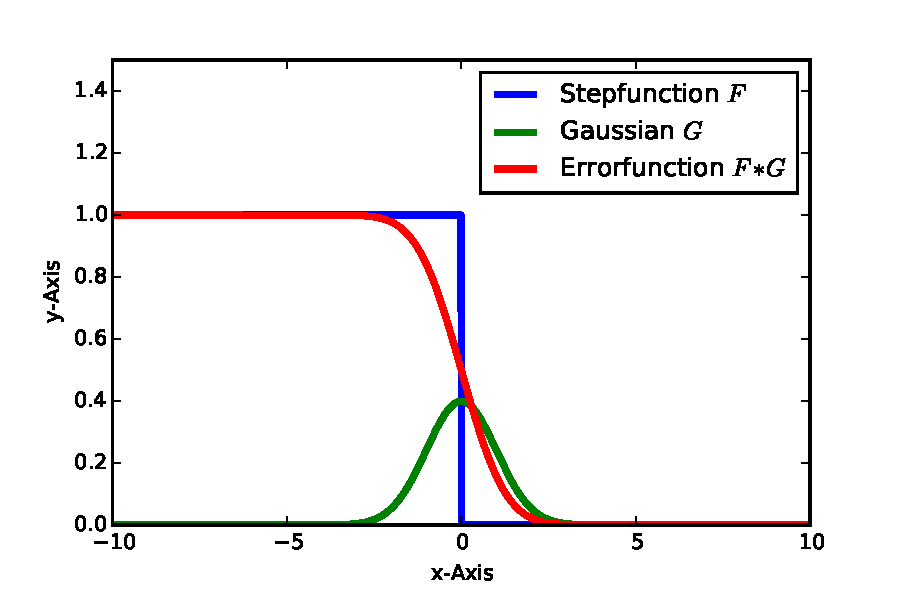
\includegraphics[width=0.75\textwidth]{plots/convolve.pdf}
	\caption{Faltung einer Kante (Stufenfunktion) mit einer Arrayscheibe (hier durch eine Gauß'sche Funktion genähert). Aus dem diskreten Sprung wird ein Gradient (in diesem Beispiel die Errorfunktion).}\label{fig:convolution}
\end{figure}
Liegen zwei Punkte zu dicht beieinander so überlappen sich ihre Arrayscheiben, und die Punkte können nicht mehr aufgelöst werden.\\
Die minimale Distanz, die zwei Punkte voneinander haben müssen, um als zwei Punkte erkannt zu werden, wird durch Auflösungskriterien bestimmt.
Das Sparrow'sche Auflösungskriterium \cite{sparrow} besagt, dass zwei Punkte (im Original Sterne) dann noch aufgelöst werden können, wenn die Intensitätsverteilung zwischen zwei Maxima gerade noch ein Minimum aufweist.
Eine konservativere Definition eines Auflösungskriteriums ist hingegen das Rayleighkriterium, welches in diesem Versuch hauptsächlich benutzt wird.
Nach Rayleigh werden zwei Punkte genau dann noch aufgelöst, wenn das Maximum eines Punktes in das Minimum des anderen fällt \cite{Dem2}.
Dies entspricht dem Abstand des ersten Minimums der PSF vom ersten Maximum und ist gegeben durch die Formel \ref{eq:rayleigh}
\begin{align}
	d_{min} = 1.22\cdot \frac{\lambda}{2n\sin \alpha}. \label{eq:rayleigh}
\end{align}
Hierbei beschreibt $\lambda$ die Wellenlänge des zu Mikroskopieren verwendeten Lichts, $n$ den Brechungsindex des Mediums und $\alpha$ den maximalen Öffnungswinkel der Obejktivlinse.
Der Term $n\sin\alpha$ wird als die numerische Apertur eines Objektivs $NA$ bezeichnet \cite{Born}.
\\
Experimentell ist die Auflösung nach Rayleigh oder Sparrow nur schwer zu messen. 
Als Maß für die Auflösung kann jedoch die Halbwertsbreite der PSF (FWHM, \emph{full width at half maximum}) benutzt werden. 
%• Erklärung Fluoreszenz und Fluoreszenzmikroskopie mit Jablonski-Diagramm.
\subsection{Fluoreszenzmikroskopie}
\begin{figure}
	\centering
	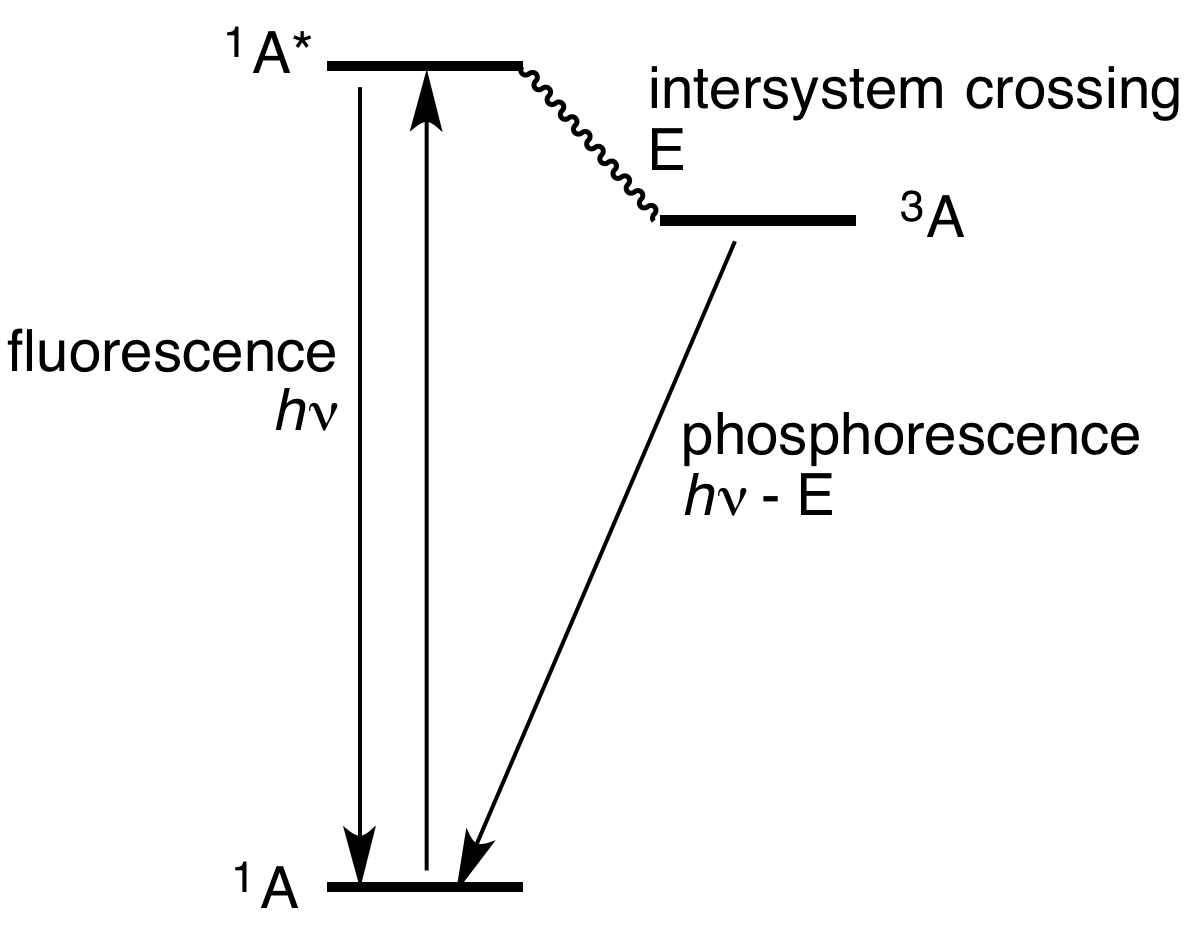
\includegraphics[width=0.6\textwidth]{plots/jablonski.png}
	\caption{Jablonski-Diagramm. (Quelle: en.wikipedia.org)}\label{fig:jablonski}
\end{figure}
Eine besondere Art von Lichtmikroskopie ist die Fluoreszenzmikroskopie.
Im Gegensatz zur klassischen Mikroskopie wird nicht, das von der Probe reflektierte oder an der Probe gebrochene Licht im Okular detektiert, vielmehr wird die Probe selbst zum Leuchten angeregt.
Das Prinzip der Fluoreszenz besteht darin Moleküle mithilfe von Licht einer spezifischen Wellenlänge in einen energetisch höheren Zustand zu versetzen. 
Bei der Rückkehr der Moleküle in ihren Grundzustand senden diese Photonen aus. 
Die Wellenlänge der absorbierten und emittierten Photonen hängt von der Verteilung der Energieniveaus des Moleküls ab. Sie ist in sogenannten Jablonski-Diagrammen schematisch dargestellt (siehe Abb. \ref{fig:jablonski}).
In der Regel befindet sich ein angeregtes Molekül nicht nur in einem elektronisch angeregten Zustand sondern auch in einem angeregten Schwingungszustand.
Durch die Relaxation aus dem Schwingungszustand besitzt das Molekül eine geringere Energie vor der Emission eines Photons als unmittelbar nach der Anregung.
Dies führt dazu, dass emittiertes Licht eine größere Wellenlänge hat als absorbiertes Licht. Dieses Phanomen trägt den Namen Stokes-Shift \cite{haken}.
\\
Der Vorteil der Fluoreszenzmikroskopie gegenüber der herkömmlichen Lichtmikroskopie ist, dass gezielt Strukturen mit Fluoreszenzfarbstoff präpariert werden können (über Proteine u.ä.) und ungewollte Brechungszentren ausgeblendet werden können.
Durch im Strahlengang eingesetzte Farbfilter wird gewährleistet, dass lediglich die emittierte Wellenlänge in das Objektiv gelangt und reflektiertes Licht abgeschrimt wird.
%• Konfokal-Mikroskopie: gehen Sie hier bitte kurz auf die Rolle der Lochblende ein
\subsection{Konfokalmikroskopie}
Eine Form der Fluoreszenzmikroskopie ist die Konfokalmikroskopie. 
Konfokalmikroskopie beleuchtet meist mit einem fokusierten Laser nur einen kleinen Ausschnitt der Probe. Allerdings wird die gesamte Probe abgerastert, sodass erst nach dem Zusammenfügen der einzelnen Flecken ein vollständiges Bild entsteht.
\\
Das Besondere an der Konfokalmikroskopie ist eine im Detektionsstrahlengang eingebrachte Lochblende. Ihre Funktion ist die Abschirmung von Licht, welches nicht von der Fokusebene stammt. Dadurch ist es möglich einen hohen Kontrast zu erzielen und nur einen scharfen Ausschnitt einer Ebene der Probe aufzunehmen.
\\
Die axiale Auflösung eines Konfokalmikroskops ist durch Gleichung (\ref{eq:axial}) bestimmt \cite{beyer}.
\begin{align}
	d_{axial} = \frac{0.88\cdot \lambda_{ex}}{n-\sqrt{n^2-NA^2}}. \label{eq:axial}
\end{align}
Hier bezeichnet $\lambda_{ex}$ die Wellenlänge der Fluoreszenzanregung. 
Die Dicke der beleuchteten Schicht lässt sich nach Gleichung (\ref{eq:slice}) bestimmen \cite{beyer}.
\begin{align}
	d_{schicht} = \sqrt{\left( \frac{0.88\lambda_{ex}}{n-\sqrt{n^2-NA^2}}\right)^2 + \left( \frac{\sqrt{2}\cdot n \cdot PH}{NA}\right)^2}. \label{eq:slice}
\end{align}
$PH$ bezeichnet den Durchmeser der konfokalen Lochblende.
%und nennen die zu erwartende Tiefendiskriminierung.
%• Beugungsgrenze in der Mikroskopie, Airy-Scheibe, beugungsbegrenzte PSF (rigo-
%rose Herleitung nicht nötig!), die Sie später für die Auswertung benötigen, Auflö-
%sungskriterien Rayleigh, Sparrow und axiale Auflösung.
%• STED-Mikroskopie: Erklärung des zugrundeliegenden Prinzips zur Auflösungs-
%erhöhung mit eigenen Worten (wichtig!).
\subsection{STED-Mikroskopie}
Die STED-Mikroskopie bietet eine Möglichkeit, die ansonsten in der Lichtmikroskopie auftretende Begrenzung der Auflösung durch Beugung zu umgehen.
Sie basiert auf der Fluoreszenzmikroskopie, und wird häufig mit einem konfokalen Aufbau realisiert.
\\
STED steht für \emph{stimulated emission depletion}, und bezieht sich auf die Abregung von Fluoreszenzmolekülen durch das Prinzip der stimulierten Emission. 
Im Gegensatz zur konventionellen Fluoreszenzmikroskopie, kommen zwei Laser unterschiedlicher Wellenlängen zum Einsatz \cite{hell}. 
Der Anregungslaser verfügt über eine PSF wie sie auch in der herkömmlichen Konfokalmikroskopie angewendet wird, i.e. eine gewöhnliche Airyscheibe.
Hinzu kommt nun ein Abregungslaser oder STED-Laser, dessen PSF die Form eines Ringes hat. Die Wellenlänge des STED-Lasers ist dabei größer als die des Anregungslasers.
Die PSFs beider Laser sind so überlagert, dass das Maximum der Anregung im Mittelpunkt des Ringes liegt.
\\
Der Anregungslaser regt Moleküle auf ein höheres Energieniveau an, die daraufhin unter Aussendung von Photonen wieder in ihren Grundzustand zurückkehren.
\\
Durch stimulierte Emission, lässt sich die Photonemission einer spezifischen Wellenlänge kontrolliert herbeiführen.
Interagiert ein angeregtes Elektron des Moleküls mit einem Photon dessen Wellenlänge dem Übergang zu einem niedrigeren Energieniveau entspricht, so fällt das Elektron in diesen Zustand unter Aussendung eines weiteren Photons dieser Wellenlänge.
\\
Dieses Prinzip wird durch den STED-Laser angewendet. Dadurch werden Moleküle aus dem Ring wieder abgeregt.
Da die Moleküle jedoch in der Regel in einen vibronischen Zustand fallen, können diese nicht sofort wieder durch den Anregungslaser zur Fluoreszenz angeregt werden.
So werden gezielt Fluoreszenzmoleküle um einen Punkt herum ausgeschaltet.
Als direkte Folge der Ratengleichungen nimmt die Anzahl der ausgeschalteten Moleküle mit steigender Intensität des STED-Lasers $I_{STED}$ exponentiell ab \cite{hell_exp}.
Die STED-Intensität bei der die Hälfte aller angeregten Moleküle ausgeschaltet wurde wird als Sättigungsintensität $I_S$ bezeichnet.
\\
Detektiert wird jetzt nur das von den verbleibenden fluoreszierenden Molekülen ausgesendete Licht. 
Es kann gezeigt werden, dass der Durchmesser der Scheibe, in der die Moleküle nicht abgeregt werden, mit steigender Intensität des STED-Lasers abnimmt \cite{hell}.
\begin{align}
	d = \frac{\lambda_{ex}}{2NA\sqrt{1+I_{STED}/I_S}}. \label{eq:sted_res}
\end{align}
Dies ermöglich eine theoretisch unbegrenzt gute Auflösung, deren Grenze nur durch die Leistung des STED-Lasers und der räumlichen Ausdehung eines Fluoreszenzmoleküls festgelegt ist.

%• Motivation / Definition des Sättigungsfaktors aus den Ratengleichungen von An-
%regung und stimulierter Emission.
%• Skalierung der Auflösung mit der Intensität.
%• Die Theorie soll sich auf gepulste Systeme beziehen, der Fall mit Dauerstrichla-
%sern ist leider nicht analytisch lösbar, aber in den experimentellen Ergebnissen
%vergleichbar.

%Kovalente Bindungen und Wasserstoffbrückenbindung
%Simulationsvereinfachungen, Ladung
%Proteinaufbau (Primär, Sekundär, Tertiärstruktur)
%Siede, und Schmelzpunkte???
% Principle Component Analysis
\section{Aufbau}
Der Versuchsaufbau besteht aus einer \SI{20}{\centi\meter} hohen Box, gefüllt mit Wasser. 
Am Boden der Zelle befindet sich eine Heizplatte, die eine Temperatur von ca. \SI{20}{\celsius} besitzt.
Nach oben hin wird die Zelle durch eine ca. \SI{10}{\celsius} kalte Kühlplatte begrenzt. \\
Zur Messung der Temperatur werden Halbleiter-Thermistoren verwendet, die einen temperaturabhängigen Widerstand besitzen. Mit der über die Thermistoren abfallenden Spannung kann die Temperatur bestimmt werden.
\\
Zum Einsatz kommt ein Thermistor im Zentrum der Konvektionszelle, dessen Höhe verstellt werden kann.
Außerdem kann die Temperatur an mehreren Stellen gleichzeitig über ein Thermistorarray an der Seite der Zelle gemessen werden. 
Das Thermistorarray besteht aus sechs Thermistoren mit einem Abstand von \SI{3}{\centi\meter}, wobei der Abstand der mittleren beiden Thermistoren \SI{4}{\centi\meter} beträgt.


\section{Durchführung}
%Gromacs programm beschreibung
%Topologie Files and PDB
%Benutzte Algorithmen
%Benutzte Parameter (Boxsize, Number of Particles, benutzte Proteine)
%
\section{Durchführung}
Das Phänomen der Rayleigh-Benard-Konvektion wird sowohl numerisch als auch experimentell untersucht.
\subsection{Simulation}
Mithilfe des Programms \emph{Comsol Multiphysics} wird die Rayleigh-Benard-Konvektion in einer zweidimensionalen Box simuliert. 
Die Simulation wird für die Rayleigh-Zahlen $10^3, 10^4, 10^5$ und $10^6$ durchgeführt. 
Ausgegeben werden dabei die Temperatur- und Geschwindigkeitsprofile entlang der Achse durch die Mitte der Box.
\\
Zudem wird die Nusselt-Zahl als das Integral des Wärmegradienten über die Grenzfläche der Box bestimmt.

\subsection{Experimentelle Betrachtung}
\subsubsection{Schattenwurfmethode}
Zunächst wird die Dynamik des Fluids im Versuchsaufbau, visuell beschrieben.
Dazu wird die Glasbox so beleuchtet, dass auf einer Seite durch die Plumes erzeugte Schatten zu erkennen sind.
Die Schatten entstehen durch die Brechung des Lichts an starken Dichtegradienten des Fluids, die Folge von Temperaturunterschieden sind.
\\
Die Geschwindigkeit der Plumes wird mithilfe einer Stoppuhr gemessen. 
Es werden sowohl auf einer Seite aufsteigende warme Plumes, als auch auf der anderen Seite fallende kalte Plumes gemessen.
\\
Die Strecke über die gemessen wird beträgt ca. 2.5~cm. Für jede Seite werden 10 Messwerte gesammelt.
\subsubsection{Beweglicher Thermistor}
Das Temperatur- und Geschwindigkeitsprofil des Fluids wird nun mit einem einzelnen Thermistor bestimmt.
Der Thermistor wird zunächst direkt an der warmen Platte in der Mitte der Box positioniert. 
Mit einem bereitgestellten Messprogramm werden nun 2048 Messwerte der Temperatur mit einer Abtastfrequenz von 9.5~Hz auf genommen. 
\\ 
Dann wird der Thermistor um 1~cm nach oben verschoben, und eine Messung für die neue Höhe gestartet. Dies wird bis zu einer Höhe von 10~cm durchgeführt.
\\
Für die ersten 1.5~cm werden die Messungen alle 0.1~cm durchgeführt. 
Für die Bestimmung der thermischen Grenzschicht wird zudem eine noch höhere Auflösung benötigt, weswegen zusätzliche Messwerte bei 0.05, 0.15, 0.25 und 0.35~cm aufgenommen werden, die allerdings nur aus 512 Messpunkten bestehen.

\subsubsection{Thermistorarray}
Anschließend wird eine lange Messung mit einem Thermistorarray aus sechs Thermistoren durchgeführt.
Mit allen Thermistoren wird über 30~Stunden hinweg die Temperatur gemessen.
Aus der zeitlichen Korrelation der Messwerte der einzelnen Thermistoren lässt sich die Geschwindigkeit von Plumes bestimmen.


\section{Auswertung}
\section{Auswertung}
%	 RAYLEIGH ZAHL DES EXPERIMENTS

% ICH	 SCHATTENPROJEKTION GESCHWINDIGKEIT 

%	 STÖRFREQUENZEN
%		FORMEL

% ICH	 TEMPERATUR ALS ABSTAND DER PLATTE

% ICH	 TEMPERATUR PROFILE

% ICH	 TEMPERATUR DURCH LANGE MESSUNG

%	 GESCHWINDIGKEITSPROFIL DURCH ABBRUCHFREQUENZ

% NUR ICH:
%	GESCHWI VERGlEICH FALL, REIBUNG
%	HISTOGRAMME TEMPERATUR

%Kondensation von Argon
% Energieplots Temperaturplot verschiedene Abkühlzeiten auf differenzen der Siedepunkte achten.
%
%Gefrieren von Argon
% Diffusionskonstante
% Radialplot
% Gefrierpunkt
%
% Simulation eines kleinen Proteins
%   RMS anstieg und fluktuation, Unterschied zur Anleitung (algorithmus)
%   Secondary structure entwicklung
%   Gyration Radius
%   Solvent accessible surface

% PCA of Lysozyme
%
\section{Diskussion}
\section{Diskussion}
\subsection{Schattenwurfmethode}
Die Schattenwurfmethode ermöglicht eine sehr simple Bestimmung der Geschwindigkeit in der Zelle. Allerdings erlaubt sie keine Bestimmung eines Geschwindigkeitsprofils. 
Sie eignet sich jedoch um die Größenordnung der in der Zelle herrschenden Geschwindigkeiten zu schätzen.
\\
Dadurch, dass die Konvektionszelle schräg präpariert wurde, sodass die Richtung der Konvektionswalze bei jedem F-Praktikumsversuch gleich ist, tritt ein systematischer Fehler auf.
Es können nicht beide Seiten der Walze gleichzeitig scharfgestellt werden.
Dadurch kommt es zu einer Überschätzung der Geschwindigkeit auf der unscharfen Seite der Zelle (bei uns die Seite der fallenden Plumes). 
Aufgrund des schelchteren Kontrastes werden nur die dunkelsten Plumes erkannt. Diese aber sind gleichzeitig die Plumes der größten Temperaturdifferenz zu ihrer Umgebung, und dadurch auch die schnellsten.
\\
Bereits im Vorraus des Versuches lässt sich die Größenorndung der Geschwindigkeiten eingrenzen. Die Obergrenze entspricht dem freien Fall mit der Beschleunigung $g\alpha\Delta T$. Über \SI{20}{\centi\meter} führt dies zu einer Geschwindigkeit von \SI{9.1}{\centi\meter\per\second}. 
Nach unten hin ist die Geschwindigkeit durch die Navier-Stokes-Gleichung beschränkt. Eine Dimensionsanalyse des Kräftegleichgewichts liefert eine Untergrenze von \SI{5e-3}{\centi\meter\per\second}. Dies enspricht auch dem Ergebnis der Geschwindigkeit im diffusiven Regime in \cref{fig:vprof_Ra_1e3}.
\\
Der gemessene Wert von \SI{0.50\pm0.01}{\centi\meter\per\second} liegt damit im erwarteten Bereich.

\subsection{Temperaturprofile}
Das mit dem beweglichen Thermistor bestimmte Temperaturprofil spiegelt das erwartete Profil gut wieder.
Ein lineares Verhalten in der Grenzschicht ist deutlich zu erkennen. Auch der konstante Temperaturverlauf im Zentrum der Zelle ist erkennbar (siehe \cref{fig:temp-prof}).
Die große Standardabweichung der Messwerte nah an der Heizplatte wird durch Plumes verursacht. 
Diese haben vor allem nah an der Heizplatte eine stark unterschiedliche Temperatur im Vergleich zur theroretischen Umgebungstemperatur des Thermistors.
Verlässt man die Grenzschicht so verringert sich auch die Fluktuation der Temperatur durch Plumes.
\\
Der Vergleich der 30-stündigen Temperaturmessung mit der Messung des beweglichen Transistors, liefert eine gute Übereinstimmung bezüglich der Konstanz der Temperatur im Zentrum der Zelle.
Allerdings sind die Messwerte der Thermistorarrays geringfügig kleiner als die des einzelen Thermistors. 
Dies kann durch eine Reihe von Gründen verursacht worden sein, von technischen Unterschieden zwischen Array und Einzelthermistor bis hin zur Temperaturschwankung durch den Tag-Nacht-Zyklus.
Der wahrscheinlichste Grund für den niederigeren Wert stammt jedoch daher, dass die für die Array-Messung verwendeten Messwerte von einem früheren F-Praktikumspaar stammen.
\\
Die numerisch erzeugten Temperaturprofile zeigen die Abhängigkeit der Rayleigh-B\'enard-Konvektion von der Rayleighzahl klar auf. 
Der Überschlag von diffusiver zu konvektiver Wärmeleitung bei Übergang von $\text{Ra}=10^3$ zu $\text{Ra}=10^4$ ist sehr deutlich zu erkennen.
Anzumerken ist jedoch, dass die Temperatur mit Abstand der Heizplatte leicht anwächst für $\text{Ra} = 10^4$ und $\text{Ra} = 10^5$.
\\
\cref{fig:hist} zeigt die Schwankungen der Temperatur in der Nähe der Grenzschicht überaus gut auf. Im Zentrum der Zelle scheinen die Messwerte normalverteilt zu sein. Je näher man allerdings zum Rand der Zelle gelangt des länger wird der Schwanz der Verteilung. Der Median trennt sich vom Maximum der Verteilung. 
Dies stimmt auch mit der Beobachtung der großen Standardabweichung in Nähe der Grenzschicht in \cref{fig:temp-prof} überein.

\subsection{Geschwindigkeitsprofile}
Das über die Frequenzanalyse bestimmte Geschwindigkeitsprofil folgt dem erwarteten Profil relativ gut. Ein Problem jedoch ist die Messung einer Geschwindigkeit während der Thermistor in Kontakt mit der Heizplatte ist. Vermutlich wird dies durch die endliche Ausdehnung des Thermistors ermöglicht, da dies die Auflösung der Messung verschlechtert.
Trotz dieses Problems lässt sich noch eine Grenzschicht im Geschwindigkeitsprofil erkennen, wie es in \cref{fig:v_prof_fc} durch den linearen Fit verdeutlich wird.
\\
Noch problematischer scheint auf den ersten Blick die Geschwindigkeitsmessung durch die Korrelation zu sein.
Das so ermittelte Profil ähnelt den simulierten Profilen in keinster Weise. Der Grund für diese Form des Profils ist jedoch eng mit dem Problem der Schattenwurfmethode verbunden.
Zunächst befindet sich das Thermistorarray nicht im Zentrum der Zelle sondern wesentlich näher am Rand. 
Dadurch befindet es sich zwangsläufig in entweder einem Aufstrom oder Abstrom (in diesem Fall einem Aufstrom) der Walze.
Bei der gemessenen Geschwindigkeit handelt es sich also nur um die Geschwindigkeit aufsteigender Plumes.
Diese kühlen jedoch auf dem Weg nach oben ab. 
Kühlere Plumes haben weniger Einfluss auf die gesamte Korrelationsfunktion. 
Die Plumes, die an den oberen Thermistoren jedoch noch mit hoher Auflösung erkannt werden, sind die wärmsten Plumes und damit die schnellsten.
So wird mit dieser Methode keine symmetrische Geschwindigkeitsverteilung gemessen.

\subsection{Bestimmung der Nusseltzahl}
Für Rayleighzahlen ab $\text{Ra} = 10^5$ stimmen die Ergebnisse für die Nusseltzahl für die Grenzschichtmethode und die Integralmethode gut überein. Die einzige Abweichung ist bei kleineren Rayleighzahlen (hier nur $10^4$) festzustellen. Die relative Abweichung des Integralergebnisses vom Grenzschichtergebnis beträgt dabei ca. 25~\%.
Betrachtet man die Temperaturprofile in \cref{fig:sim-temp} so lässt sich vermuten, dass die Grenzschichtmethode bei kleinen Rayleighzahlen ungenauer wird, da das lineare Regime der Temperatur schwerer einzugrenzen ist.
\\
Insgesamt ergibt sich allerdings ein guter Wert für den Exponenten im ermittelten Potenzgesetz. In der Literatur wird hier ein Wert von $0.309$ \cite{expo} damit eine relative Abweichung von ca. 16~\%. 






\bibliography{master}
\end{document}
